% A strongly connected digraph of period 3: the classes {1,2}, {3,4,5}, {6,7} are visited cyclically.
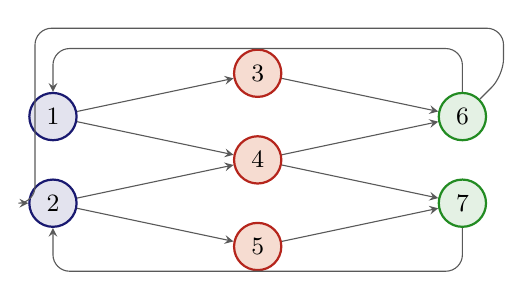
\begin{tikzpicture}[>=stealth,scale=1.0]
\node[circle,draw=MidnightBlue,fill=MidnightBlue!12,thick,minimum size=6mm,font=\small] (v1) at (0.000,0.550) {$1$};
\node[circle,draw=MidnightBlue,fill=MidnightBlue!12,thick,minimum size=6mm,font=\small] (v2) at (0.000,-0.550) {$2$};
\node[circle,draw=BrickRed,fill=BrickRed!12,thick,minimum size=6mm,font=\small] (v3) at (2.600,1.100) {$3$};
\node[circle,draw=BrickRed,fill=BrickRed!12,thick,minimum size=6mm,font=\small] (v4) at (2.600,-0.000) {$4$};
\node[circle,draw=BrickRed,fill=BrickRed!12,thick,minimum size=6mm,font=\small] (v5) at (2.600,-1.100) {$5$};
\node[circle,draw=ForestGreen,fill=ForestGreen!12,thick,minimum size=6mm,font=\small] (v6) at (5.200,0.550) {$6$};
\node[circle,draw=ForestGreen,fill=ForestGreen!12,thick,minimum size=6mm,font=\small] (v7) at (5.200,-0.550) {$7$};
\draw[->,black!65] (v1) -- (v3);
\draw[->,black!65] (v1) -- (v4);
\draw[->,black!65] (v2) -- (v4);
\draw[->,black!65] (v2) -- (v5);
\draw[->,black!65] (v3) -- (v6);
\draw[->,black!65] (v4) -- (v6);
\draw[->,black!65] (v4) -- (v7);
\draw[->,black!65] (v5) -- (v7);
\draw[->,black!65,rounded corners=6pt] (v6.north) -- ++(0,0.55) -| (v1.north);
\draw[->,black!65,rounded corners=6pt] (v6.north east) -- ++(0.3,0.3) -- ++(0,0.6) -- ++(-5.95,0) |- (v2.west);
\draw[->,black!65,rounded corners=6pt] (v7.south) -- ++(0,-0.55) -| (v2.south);
\end{tikzpicture}
